%!TEX TS-program = xelatex
%!TEX encoding = UTF-8 Unicode
% Awesome CV LaTeX Template for CV/Resume
%
% This template has been downloaded from:
% https://github.com/posquit0/Awesome-CV
%
% Author:
% Claud D. Park <posquit0.bj@gmail.com>
% http://www.posquit0.com
%
%
% Adapted to be an Rmarkdown template by Mitchell O'Hara-Wild
% 23 November 2018
%
% Template license:
% CC BY-SA 4.0 (https://creativecommons.org/licenses/by-sa/4.0/)
%
%-------------------------------------------------------------------------------
% CONFIGURATIONS
%-------------------------------------------------------------------------------
% A4 paper size by default, use 'letterpaper' for US letter
\documentclass[11pt,a4paper,]{awesome-cv}

% Configure page margins with geometry
\usepackage{geometry}
\geometry{left=1.4cm, top=.8cm, right=1.4cm, bottom=1.8cm, footskip=.5cm}


% Specify the location of the included fonts
\fontdir[fonts/]

% Color for highlights
% Awesome Colors: awesome-emerald, awesome-skyblue, awesome-red, awesome-pink, awesome-orange
%                 awesome-nephritis, awesome-concrete, awesome-darknight

\definecolor{awesome}{HTML}{6767C7}

% Colors for text
% Uncomment if you would like to specify your own color
% \definecolor{darktext}{HTML}{414141}
% \definecolor{text}{HTML}{333333}
% \definecolor{graytext}{HTML}{5D5D5D}
% \definecolor{lighttext}{HTML}{999999}

% Set false if you don't want to highlight section with awesome color
\setbool{acvSectionColorHighlight}{true}

% If you would like to change the social information separator from a pipe (|) to something else
\renewcommand{\acvHeaderSocialSep}{\quad\textbar\quad}

\def\endfirstpage{\newpage}

%-------------------------------------------------------------------------------
%	PERSONAL INFORMATION
%	Comment any of the lines below if they are not required
%-------------------------------------------------------------------------------
% Available options: circle|rectangle,edge/noedge,left/right

\photo{../images/MVA.jpg}
\name{Milena}{Vásquez-Amézquita}

\position{Associate Professor}
\address{Faculty of Psychology, Universidad El Bosque}

\mobile{(+57) 601-6489000 Ext. 1605}
\email{\href{mailto:mvasquezam@unbosque.edu.co}{\nolinkurl{mvasquezam@unbosque.edu.co}}}
\homepage{grupo-codec.netlify.app/author/milena-vasquez-amezquita/}
\orcid{0000-0001-7317-8430}
\googlescholar{XgNEpfgAAAAJ}
\researchgate{Milena-Vasquez-Amezquita}

% \gitlab{gitlab-id}
% \stackoverflow{SO-id}{SO-name}
% \skype{skype-id}
% \reddit{reddit-id}

\quote{I am a researcher primarily interested in the neurocognitive
bases of human affect and sexuality.}

\usepackage{booktabs}

\providecommand{\tightlist}{%
	\setlength{\itemsep}{0pt}\setlength{\parskip}{0pt}}

%------------------------------------------------------------------------------



% Pandoc CSL macros

\begin{document}

% Print the header with above personal informations
% Give optional argument to change alignment(C: center, L: left, R: right)
\makecvheader

% Print the footer with 3 arguments(<left>, <center>, <right>)
% Leave any of these blank if they are not needed
% 2019-02-14 Chris Umphlett - add flexibility to the document name in footer, rather than have it be static Curriculum Vitae
\makecvfooter
  {27 May, 2024}
    {Milena Vásquez-Amézquita~~~·~~~Academic Curriculum Vitae}
  {\thepage}


%-------------------------------------------------------------------------------
%	CV/RESUME CONTENT
%	Each section is imported separately, open each file in turn to modify content
%------------------------------------------------------------------------------



\section{About me}\label{about-me}

\begin{minipage}[c]{0.85\linewidth}
Psychologist, Master in Basic and Applied Neurosciences and PhD in Neurosciences. Active associate researcher within the group \href{https://investigaciones.unbosque.edu.co/codec}{\textit{\textbf{CODEC}: Cognitive and Behavioural Sciences}} (classification \href{https://scienti.minciencias.gov.co/gruplac/jsp/visualiza/visualizagr.jsp?nro=00000000001446}{\textbf{A1}} in MinCiencias). Associate Professor at the \href{https://grupo-codec.netlify.app/labpsiexp/}{\textbf{Laboratory of Experimental Psychology}} of the \href{https://www.uelbosque.edu.co/psicologia}{Faculty of Psychology} at \href{https://www.uelbosque.edu.co/}{Universidad El Bosque}. Postdoctoral stay at \href{https://www.cuc.edu.co/}{Universidad de la Costa} with funding from \href{https://minciencias.gov.co/}{MinCiencias}. I have been director and co-director of successful research projects from an experimental methodology in cognitive-affective neuroscience with internal and external funding, and I currently directing the research hotbed \href{https://grupo-codec.netlify.app/sexcog/}{\textit{\textbf{SexCog}: sexuality and affectivity from a neurocognitive perspective}}. I have 13 years of professional and university teaching experience, applied to the development and implementation of undergraduate and postgraduate higher education programmes related to the neurobiological and cognitive bases of human behaviour, and I have supervised undergraduate, masters and doctoral degree projects.
\end{minipage} \begin{minipage}[c]{0.15\linewidth}
\begin{flushright} 
\hfill \href{https://grupo-codec.netlify.app/sexcog/}{
\includegraphics[width=2.3cm, height=2.3cm]{Logo_SEXCOG.png}} \newline \href{https://investigaciones.unbosque.edu.co/codec}{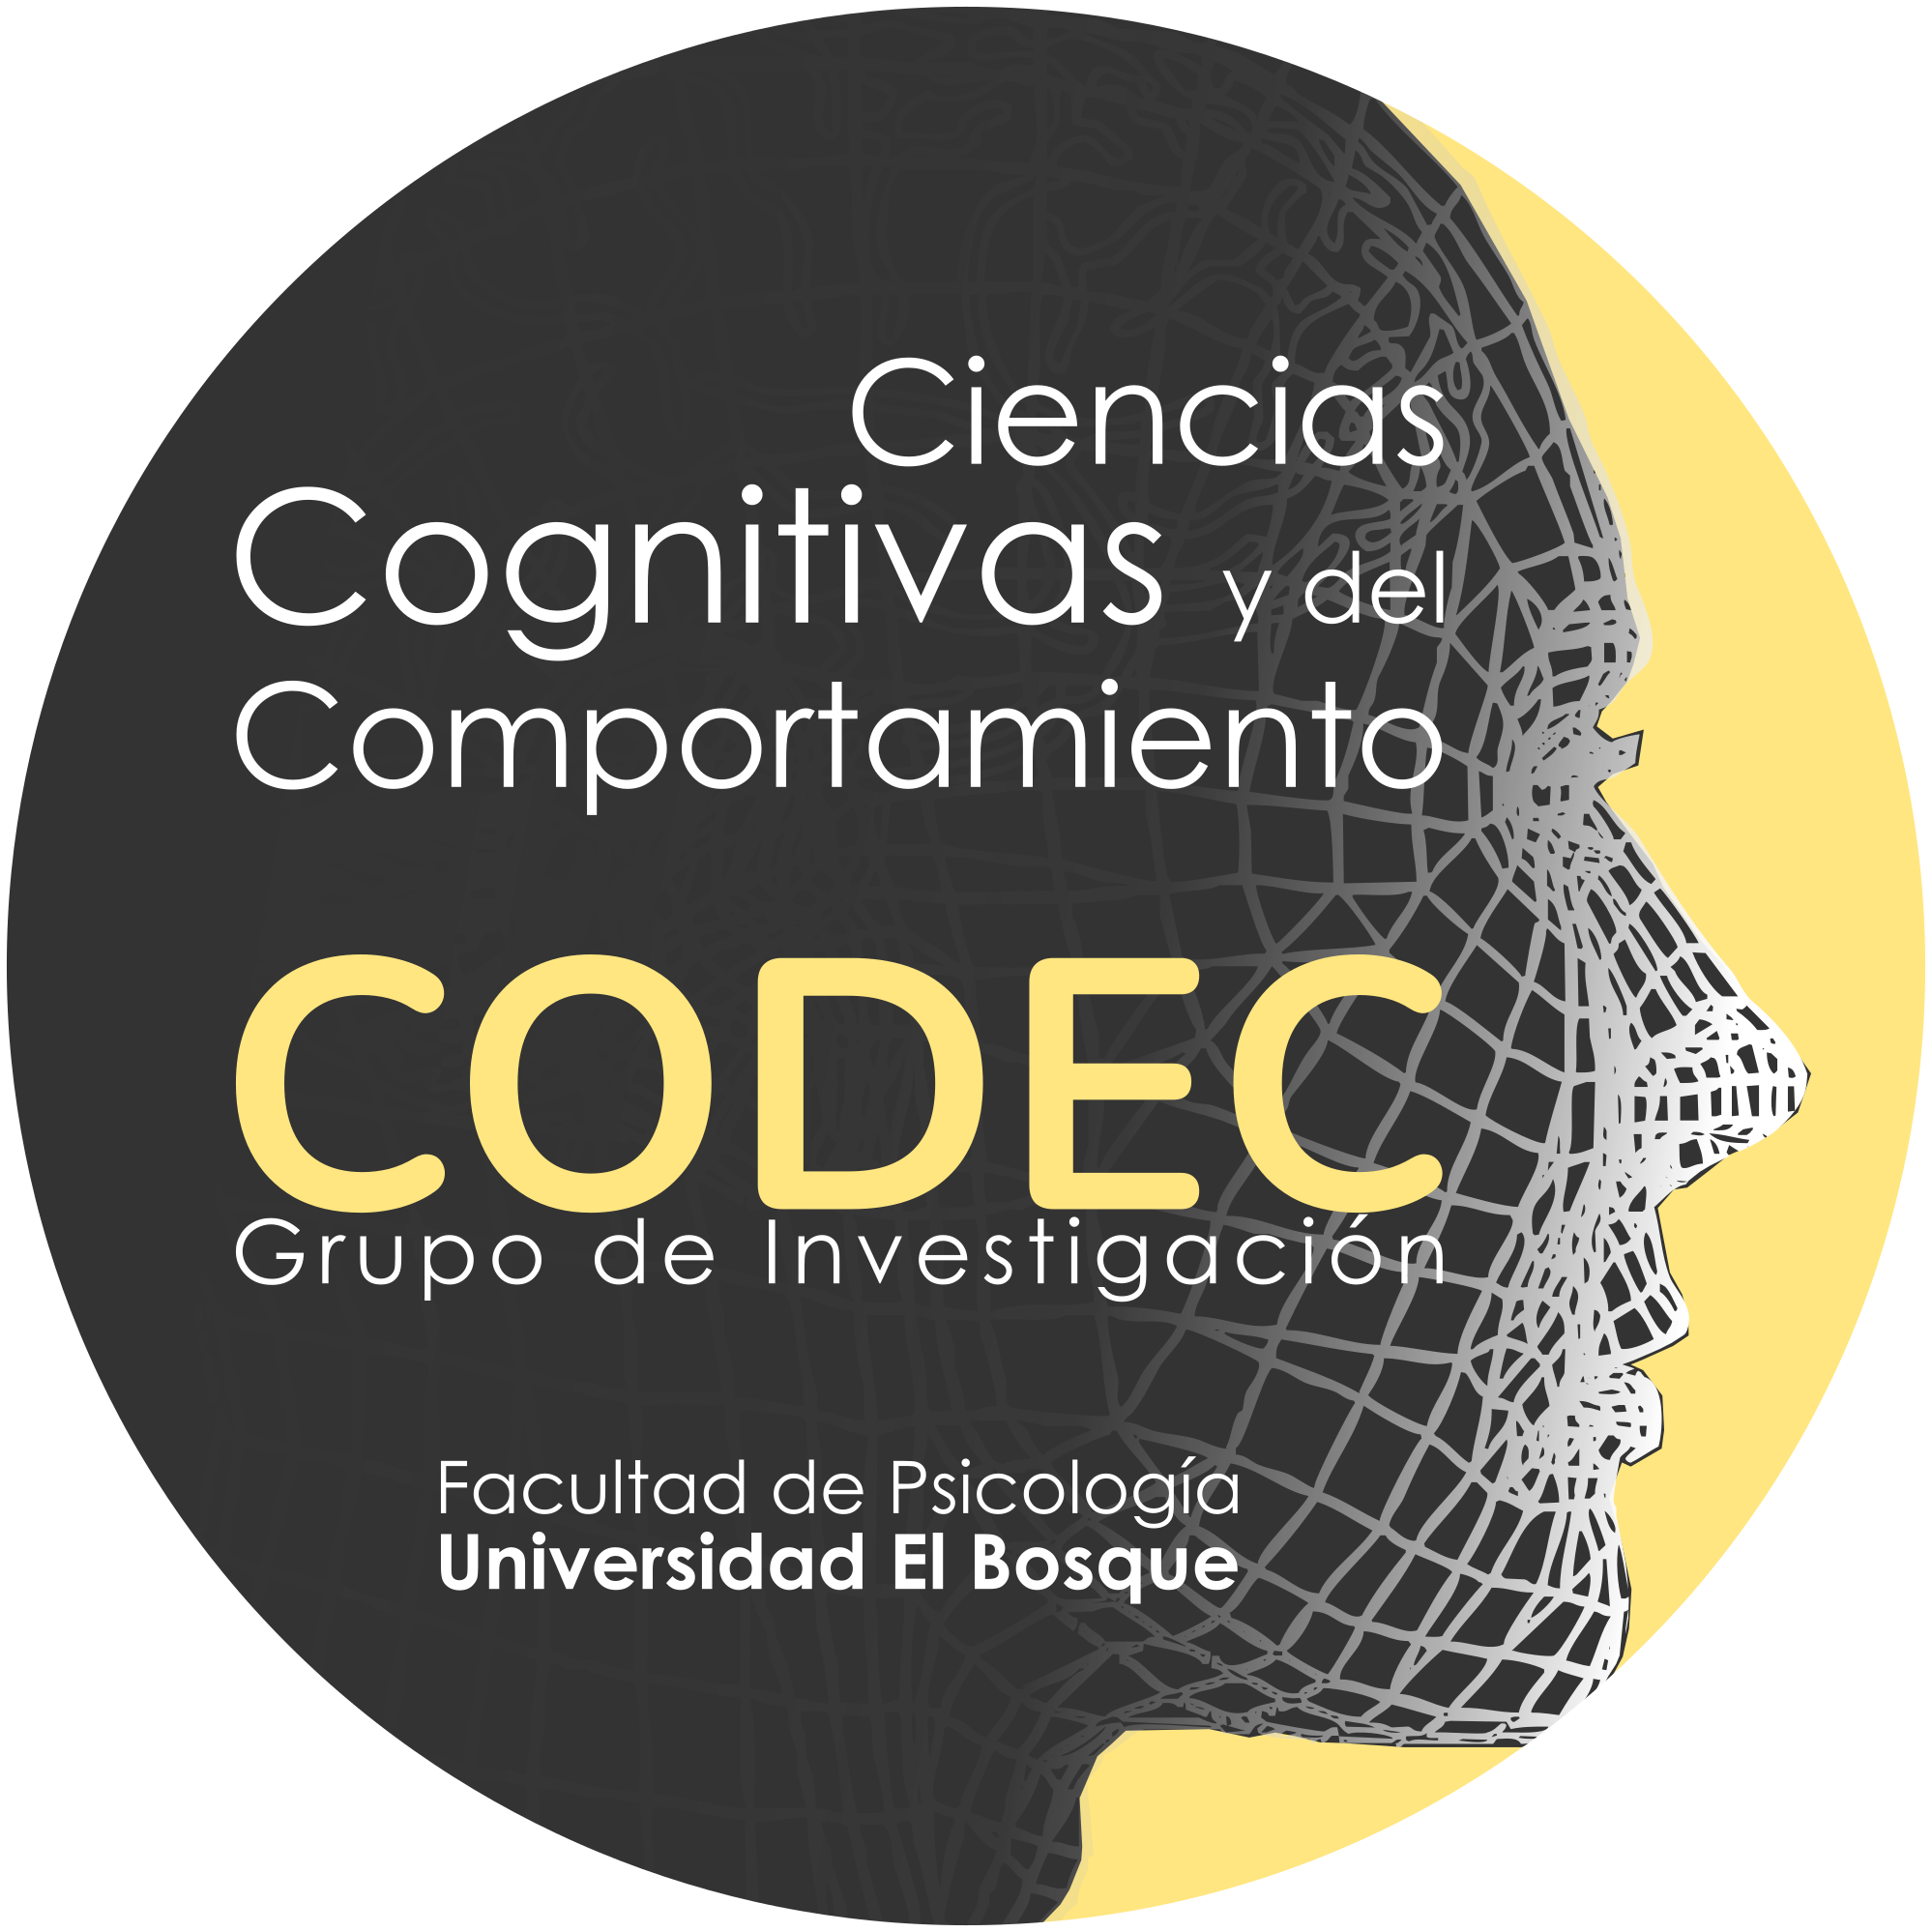
\includegraphics[width=2.3cm, height=2.3cm]{Logo_CODEC.png}}
\end{flushright}
\end{minipage}

\section{Skills}\label{skills}

\begin{cvskills}
  \cvskill
    {Programming}
    {\href{https://www.r-project.org/}{\textbf{R}} (Basic, data analysis and graph generation)}

  \cvskill
    {Quantitative Research}
    {Observational-correlational studies, Simple and Mixed general linear models}
  
  \cvskill
    {Recording techniques}
    {Eye tracking (mainly), other basic HRV, EEG}

  \cvskill
    {Software}
    {RStudio, Tobii Pro Lab, Qualtrics, Psychomorph, WebmorphR, Mendeley and Zotero}

  \cvskill
    {Languages}
    {English/Spanish (native)}
\end{cvskills}

\section{Research}\label{research}

\begin{cvskills}
  \cvskill
    {Research Areas}
    {\textbf{Human sexual response • Typical and atypical sexual preferences • Pedohebephilia • Harmful sexual \newline behaviors • Mate choice • Attentional biases}}

  \cvskill
    {Primary Research Methods}
    {Experimental designs • Free viewing \& forced stimulus choice paradigms • Psychometric scales • Subjective \newline assessment of visual stimuli}
\end{cvskills}

\section{Education}\label{education}

\begin{cventries}
    \cventry{PhD - Neurosciences}{\href{https://www.uv.es/uvweb/universidad/es/universidad-valencia-1285845048380.html}{Universidad de Valencia}}{Valencia, España}{2018}{\begin{cvitems}
\item Research project: \href{https://producciocientifica.uv.es/documentos/5eb09d10299952764112462f}{\textbf{\textit{Preferencias sexuales típicas y atípicas según sexo y edad de los estímulosutilidad de la técnica de rastreo ocular}}}
\item Supervisors: \href{https://www.uv.es/labnsc/miembros\%20individualmente/miembrosaliciasalvador.html/}{Prof. Alicia Salvador}, y \href{https://jdleongomez.info/es/}{Prof. Juan David Leongómez}
\end{cvitems}}
    \cventry{Master's Degree in Basic and Applied Neurosciences}{\href{https://www.uv.es/uvweb/universidad/es/universidad-valencia-1285845048380.html}{Universidad de Valencia}}{Valencia, España}{2012}{\begin{cvitems}
\item Research product: \href{https://revistas.um.es/analesps/article/view/analesps.31.1.167241/169861}{\textbf{\textit{Effects of assisted training with neurofeedback on EEG measures, executive function and mood in a healthy sample}}}
\item Supervisor: \href{https://www.researchgate.net/profile/Marien-Gadea}{Prof. Marien Gadea}
\end{cvitems}}
    \cventry{Psychology}{\href{https://www.ucatolica.edu.co/portal/Pregrado/psicologia/}{Universidad Cátolica de Colombia}}{Bogotá, Colombia}{2007}{\begin{cvitems}
\item Research product: \href{http://www.scielo.org.co/scielo.php?pid=S1794-99982009000200010&script=sci_arttext}{\textbf{\textit{Diseño del cuestionario de creencias referidas al consumo de alcohol para jóvenes universitarios}}}
\end{cvitems}}
\end{cventries}

\section{Relevant further education}\label{relevant-further-education}

\begin{cventries}
    \cventry{Diplomado en Diseño y Uso Pedagógico de Ambientes Virtuales de Aprendizaje Mediados por las TIC y las TAC}{Universidad El Bosque}{Bogotá, Colombia}{2020}{}\vspace{-4.0mm}
    \cventry{Diploma in University Teaching}{Politécnico Superior de Colombia}{Bogotá, Colombia}{2019}{}\vspace{-4.0mm}
\end{cventries}

\section{Academic Experience}\label{academic-experience}

\begin{cventries}
    \cventry{Associate Professor}{\href{https://www.unbosque.edu.co/}{Universidad El Bosque}}{Bogotá, Colombia}{2020 - Present}{\begin{cvitems}
\item Research Degree Project III (2020-2024)
\item Advanced Seminar II (Psychology Msc) (2020)
\end{cvitems}}
    \cventry{Assistant Professor}{\href{https://www.unbosque.edu.co/}{Universidad El Bosque}}{Bogotá, Colombia}{2015 - 2019}{\begin{cvitems}
\item Advanced Seminar II (Psychology Msc) (2019)
\item Neurosciences and Behavior Laboratory (2015 - 2019)
\item Motivation and Emotion Laboratory (2015-2019)
\item Cognitive Processes Laboratory (2015 - 2018)
\end{cvitems}}
    \cventry{Cathedratic Professor}{\href{https://www.usbbog.edu.co/}{Universidad de San Buenaventura de Bogotá}}{Bogotá, Colombia}{2015}{\begin{cvitems}
\item 
Advanced Workshop (Neuropsychology Msc)  (2019-2020)
\end{cvitems}}
    \cventry{Assistant Professor}{\href{https://www.usbmed.edu.co/}{Universidad de San Buenaventura de Medellín - Sede Ibagué}}{Ibagué, Colombia}{2013 - 2014}{\begin{cvitems}
\item Neuroscience Basics (2013 - 2014)
\item Neuropsychology I (2013 - 2014)
\item Neuropsychology II  (2013 - 2014)
\item Introduction to Practice Seminar (2013-2014)
\item Research project (2013-2014)
\end{cvitems}}
    \cventry{Cathedratic Professor}{\href{https://www.uan.edu.co/es/}{Universidad Antonio Nariño}}{Bogotá, Colombia}{2013 - 2014}{\begin{cvitems}
\item Basic Psychological Processes II- Laboratory (2014)
\item Motivation and Emotion (2014)
\item Learning and Memory (2014)
\item Neurosciences III (2014)
\item Personality Theories (2013)
\item Research Seminar IV (2013)
\item Elective Seminar IV- Sexuality, Gender and Culture (2013)
\item Research Project (2013-2014)
\end{cvitems}}
    \cventry{Cathedratic Professor}{\href{https://www.ucatolica.edu.co/}{Universidad Cátolica de Colombia}}{Bogotá, Colombia}{2009}{\begin{cvitems}
\item Functional Neuroanatomy Research Lab (2009)
\item Neuropsychology Lab  (2009)
\end{cvitems}}
\end{cventries}

\section{Research Experience}\label{research-experience}

\begin{cventries}
    \cventry{Associate Professor}{\href{https://www.unbosque.edu.co/}{Universidad El Bosque}}{Bogotá, Colombia}{Jan. 2020 - Present}{\begin{cvitems}
\item Researcher at \href{https://grupo-codec.netlify.app/people/}{Experimental Psychology Laboratory}
\item Director of the \href{https://grupo-codec.netlify.app/sexcog/}{SexCog Research Incubator}
\item Supervision of a variety of undergraduate research projects associated with psychology
\end{cvitems}}
    \cventry{Visiting Professor}{\href{https://www.cuc.edu.co/}{Universidad de la Costa}}{Barranquilla, Colombia}{Dec. 2023 - Present}{\begin{cvitems}
\item II Postdoctoral stay funding by Minciencias, Colombia
\end{cvitems}}
    \cventry{Collaborating Professor}{\href{https://www.universidadviu.com/co/maestria-universitaria-en-neuropsicologia-clinica}{Univiersidad Internacional de Valencia}}{Valencia, España}{Oct. 2023 - Present}{\begin{cvitems}
\item Supervision of Master's research projects related to clinical neuropsychology.
\end{cvitems}}
    \cventry{Visiting Professor}{\href{https://www.cuc.edu.co/}{Universidad de la Costa}}{Valencia, España}{Jan. 2021 - Jan. 2023}{\begin{cvitems}
\item I Postdoctoral stay funding by Minciencias, Colombia
\end{cvitems}}
    \cventry{Assistant Professor}{\href{https://www.unbosque.edu.co/}{Universidad El Bosque}}{Bogotá, Colombia}{Jan. 2015 - Dec. 2019}{\begin{cvitems}
\item Researcher at \href{https://grupo-codec.netlify.app/people/}{Experimental Psychology Laboratory}
\end{cvitems}}
    \cventry{Research Professor}{\href{https://www.usbmed.edu.co/}{Universidad de Sanbuenaventura de Medellín}}{Medellín, Colombia}{Jan. 2013 - Jun. 2015}{\begin{cvitems}
\item Researcher at the Psychology \& Neurosciences Research Group (2014 - 2015)
\item Supervision of a variety of undergraduate research projects associated with psychology \& Neuropsychology (2013 - 2014)
\item Neurognosis research incubator leader (2013-2014)
\end{cvitems}}
\end{cventries}

\section{Professional Experience}\label{professional-experience}

\begin{cventries}
    \cventry{External Scientific Consultant}{\href{https://www.redpapaz.org/}{ONG RedPapaz}}{Bogotá, Colombia}{Sep. - Oct. 2022}{\begin{cvitems}
\item Consultancy in the implementation of a child sexual abuse prevention project  \href{https://childhelplineinternational.org/te-guio/}{TeGuío Helpline}
\end{cvitems}}
    \cventry{International Scientific Consultant}{\href{https://www.suojellaanlapsia.fi/en}{Protect Children}}{Helsink, Finlandia}{Jul. - Aug. 2021}{\begin{cvitems}
\item Translation and adaptation into Spanish of the  \href{https://www.mielenterveystalo.fi/en/self-help/redirection-self-help-program-stop-using-csam}{Global ReDirection Program: Protecting Children Through Prevention}
\end{cvitems}}
    \cventry{Professional Validator}{\href{https://https://www.areandina.edu.co/}{Fundación del area Andina}}{Bogotá, Colombia}{Sep. 2020 - Jan.2021}{\begin{cvitems}
\item Expert validator of the selection instrument for the provision of vacant jobs in territorial calls 2019-II.
\end{cvitems}}
    \cventry{Neuropsychology Professional}{\href{https://web.facebook.com/ACYSTERAPIAS/}{Centro de Atención Terapéutica ACYS, Colombia}}{Bogotá, Colombia}{Aug. 2013 - Jan. 2021}{\begin{cvitems}
\item Neuropsychological assessment in children and adolescents
\end{cvitems}}
    \cventry{Neuropsychology Professional}{\href{https://neurolearningterapias.com/nosotros/}{Organización de Terapia Integral Pavlov, Colombia }}{Bogotá, Colombia}{Aug. 2008 - Sept. 2009}{\begin{cvitems}
\item Evaluation and training in Neurofeedback
\end{cvitems}}
\end{cventries}

\section{Grants}\label{grants}

\begin{cventries}
    \cventry{\href{https://minciencias.gov.co/convocatorias/construccion-paz-programa-y-proyectos-ctei-fortalecimiento-capacidades-para-la}{Postdoctoral Research Stays -  Call 935-2023 - Orchids Program. Women in science: agents for peace: Agents for Peace 2023}}{\href{https://minciencias.gov.co/}{Minciencias}}{Barranquilla, Colombia}{Dic. 2023 - Jan. 2025}{\begin{cvitems}
\item Project: Effect of resource availability on women's preferences for masculinity faces in interaction with hormonal, cognitive, and socio-contextual factors such as actual resource scarcity and exposure to violence: an experimental study using eye-tracking
\item COP\$356.040.884
\end{cvitems}}
    \cventry{IX \href{https://www.unbosque.edu.co/centro-informacion/convocatoria/xiv-convocatoria-interna-de-investigaciones}{Internal Call for Financing Research and Technological Innovation Projects El Bosque University}, 2024}{\href{https://www.unbosque.edu.co/}{Universidad El Bosque}}{Bogota, Colombia}{Jan. 2024 - Jan. 2026}{\begin{cvitems}
\item Project: Effect of real and simulated resource control on androphilic women's preferences for masculinity in men's faces: an experimental study using eye-tracking
\item Role: Principal Researcher
\item COP\$90.000.000
\end{cvitems}}
    \cventry{\href{https://minciencias.gov.co/convocatorias/oportunidades-formacion/convocatoria-programa-estancias-postdoctorales-en-entidades}{Call for Postdoctoral Fellowship Program in SNCTeI entities 2019}}{\href{https://minciencias.gov.co/}{Minciencias}}{Barranquilla, Colombia}{Jan. 2021 - Jan. 2022}{\begin{cvitems}
\item Project: Feasibility of new interventions to improve the implementation of sexual and reproductive health programs in Colombia.
\item COP\$192.000.000
\end{cvitems}}
    \cventry{\href{https://minciencias.gov.co/convocatorias/vocaciones-cientificas-ctei/convocatoria-para-el-fortalecimiento-proyectos-en}{Call for the strengthening of projects in execution of CTeI in health sciences with young talent and regional impact 2020}}{\href{https://minciencias.gov.co/}{Minciencias}}{Bogota, Colombia}{Jan. 2021 - Jan. 2022}{\begin{cvitems}
\item Project: Attentional biases and their relationship with heart rate variability as predictors of emotional state in people without affective disorders in the city of Bogotá.
\item Role: Principal Researcher
\item COP\$76.000.000
\end{cvitems}}
    \cventry{IX \href{https://www.unbosque.edu.co/investigaciones/convocatorias-investigacion}{Internal Call for Financing Research and Technological Innovation Projects El Bosque University}, 2017}{\href{https://www.unbosque.edu.co/}{Universidad El Bosque}}{Bogota, Colombia}{Jan. 2018 - Dic. 2021}{\begin{cvitems}
\item Project: Perceivable signs of physical and mental health in faces, voices and body odors, and their relationship to hormone levels
\item Role: Co-researcher
\item COP\$136.586.537
\end{cvitems}}
    \cventry{VII \href{https://www.unbosque.edu.co/investigaciones/convocatorias-investigacion}{Internal Call for Financing Research and Technological Innovation Projects El Bosque University}, 2015}{\href{https://www.unbosque.edu.co/}{Universidad El Bosque}}{Bogota, Colombia}{Jan. 2016 - Dic. 2019}{\begin{cvitems}
\item Project: Differences in the pattern of eye tracking to sexually preferred stimuli in men convicted of sexual offenses and the general population
\item Role: Principal Researcher
\item COP\$80.000.000
\end{cvitems}}
    \cventry{Convocatoria Interna de Investigación Financiera de la Universidad de San Buenaventura, 2014}{\href{https://www.usbmed.edu.co/}{Universidad San Buenaventura de Medellín}}{Medellín, Colombia}{Jun.2014 - Jun.2015}{\begin{cvitems}
\item Project: Mediating factors of Cognitive Reserve and its relationship with the neuropsychological profile of the older adult in the process of normal aging
\item Role: Principal Researcher
\item COP\$20.000.000
\end{cvitems}}
\end{cventries}

\section{Scholarships, Awards and
Honors}\label{scholarships-awards-and-honors}

\begin{cventries}
    \cventry{X Excellence Awards}{\href{https://www.unbosque.edu.co/}{Universidad El Bosque}}{Bogotá, Colombia}{Dic. 2023}{\begin{cvitems}
\item COP\$10.000.000
\end{cvitems}}
    \cventry{VIII Excellence Awards}{\href{https://www.unbosque.edu.co/}{Universidad El Bosque}}{Bogotá, Colombia}{Dic. 2019}{\begin{cvitems}
\item COP\$5.000.000
\end{cvitems}}
    \cventry{VII Excellence Awards}{\href{https://www.unbosque.edu.co/}{Universidad El Bosque}}{Bogotá, Colombia}{Dic. 2018}{\begin{cvitems}
\item COP\$2.500.000
\end{cvitems}}
    \cventry{Cum Laude Mention}{\href{https://www.uv.es/}{Universidad de Valencia}}{Valencia, España}{Sep. 2018}{\begin{cvitems}
\item PhD Thesis in Neurosciences
\end{cvitems}}
    \cventry{Luisa Cardona Scholarship}{\href{https://https://www.uv.es/uvcooperacion/es/becas-ayudas/ayudas-estudiantes-paises-cooperacion/becas-luisa-cardona.html/}{Universidad de Valencia}}{Valencia, España}{Nov.2011 - Nov.2012}{\begin{cvitems}
\item Fee exemption for the Official Master's Degree
\end{cvitems}}
    \cventry{Honorary Degree}{\href{https://www.ucatolica.edu.co/}{Universidad Cátolica de Colombia}}{Bogotá, Colombia}{Sep. 2007}{\begin{cvitems}
\item Improved performance among undergraduate psychology students
\end{cvitems}}
    \cventry{Mention for excellence}{\href{https://https://www.ucatolica.edu.co/portal/Facultades/facultad-de-psicologia/}{Universidad Cátolica de Colombia}}{Bogotá, Colombia}{Mar.2007}{\begin{cvitems}
\item Mention postgraduate scholarship for obtaining the highest score among the psychology students of the faculty and 3rd place nationally in the 2006 version of the Quality Examination for Higher Education in Colombia (ECAES).
\end{cvitems}}
\end{cventries}

\section{Publications}\label{publications}

\begin{tcolorbox}[enhanced,
        on line, 
        boxsep=4pt, left=0pt,right=0pt,top=0pt,bottom=0pt,
        colframe=white,colback=violet,
        hyperurl={https://scholar.google.com/citations?user=XgNEpfgAAAAJ}]
  
\color{white}
  \begin{minipage}[c]{0.245\linewidth}
    \begin{center} 
      \begin{huge} 7 \end{huge}
     \begin{small} \textit{h}-index \end{small} 
    \end{center} 
  \end{minipage} 
  \begin{minipage}[c]{0.245\linewidth}
    \begin{center} 
      \begin{huge} 19 \end{huge}
      \begin{small} \textit{g}-index \end{small} 
    \end{center}
  \end{minipage} 
  \begin{minipage}[c]{0.245\linewidth}
    \begin{center} 
      \begin{huge} 7 \end{huge}
      \begin{small} i10-index \end{small} 
    \end{center}
  \end{minipage} 
  \begin{minipage}[c]{0.245\linewidth}
    \begin{center}  
      \begin{huge} 20 \end{huge}
      \begin{small} Publications \end{small} 
    \end{center}
  \end{minipage} 
  
  \begin{center} \noindent\line(1,0){150} Citations \noindent\line(1,0){150} \end{center}
  
  \begin{minipage}[c]{0.325\linewidth}  
    \begin{center} 
      \begin{small} Total \end{small} 
      \begin{LARGE} 387 \end{LARGE} 
    \end{center}
  \end{minipage} 
  \begin{minipage}[c]{0.325\linewidth}
    \begin{center} 
      \begin{small} Mean \end{small} 
      \begin{LARGE} 19.35 \end{LARGE}
    \end{center}
  \end{minipage} 
  \begin{minipage}[c]{0.325\linewidth}
    \begin{center}  
      \begin{small} Median \end{small} 
      \begin{LARGE} 4.5 \end{LARGE}
   \end{center}
  \end{minipage} 
\end{tcolorbox}

\subsection{\texorpdfstring{\textbf{Journal Articles}}{}}\label{section}

\begingroup
\footnotesize
\setlength{\parindent}{-0.5in}
\setlength{\leftskip}{0.5in}

\textbf{Vásquez-Amézquita, M.}, Leongoméz, J. D., Salvador, A., \& Seto,
M. C. (2023). What can the eyes tell us about atypical sexual
preferences as a function of sex and age? Linking eye movements with
child-related chronophilias. \emph{Forensic Sciences Research,
8}(1)1--11. \url{https://doi.org/10.1093/fsr/owad009}

\textbf{Vásquez-Amézquita, M.}, Salvador, A., \& Leongómez, J. D.
(2021). Existen diferencias en la ratio 2D:4D entre delincuentes
sexuales y no sexuales, y hombres no delincuentes? Un estudio en una
muestra colombiana. Interdisciplinaria. \emph{Revista de Psicología y
Ciencias Afines, 39}(1).
\url{https://doi.org/10.16888/interd.2022.39.1.8}

Leongómez, J. D., Sánchez, O. R., \textbf{Vásquez-Amézquita, M.}, \&
Roberts, S. C. (2021). Contextualising courtship: Exploring male body
odour effects on vocal modulation. \emph{Behavioural Processes, 193}
104531.
\url{https://doi.org/https://doi.org/10.1016/j.beproc.2021.104531}

Jones, B. C., DeBruine, L. M., Flake, J. K., Liuzza, M. T., Antfolk, J.,
Arinze, N. C., Ndukaihe, I. L. G., Bloxsom, N. G., Lewis, S. C., Foroni,
F., Willis, M. L., Cubillas, C. P., Vadillo, M. A., Turiegano, E.,
Gilead, M., Simchon, A., Saribay, S. A., Owsley, N. C., Jang, C. \ldots,
\textbf{Vásquez-Amézquita, M.}, \ldots, Coles, N. A. (2021). To which
world regions does the valence--dominance model of social perception
apply? Nature Human Behaviour, 5(1) 159-169.
\url{https://doi.org/10.1038/s41562-020-01007-2}

Leongómez, J. D., Sanchez, O. R., \textbf{Vásquez-Amézquita, M.},
Valderrama, E., Castellanos-Chacon, A., Morales-Sanchez, L., Nieto, J.,
\& Gonzalez-Santoyo, I. (2020). Self-reported Health is Related to Body
Height and Waist Circumference in Rural Indigenous and Urbanised
Latin-American Populations. \emph{Scientific Reports, 10}, 4391.
\url{https://doi.org/10.1101/562942}

\textbf{Vásquez-Amézquita, M.}, Leongómez, J. D., Seto, M. C., Bonilla,
F. M., Rodríguez-Padilla, A., \& Salvador, A. (2018). No relation
between digit ratio (2D:4D) and visual attention patterns to sexually
preferred and non-preferred stimuli. \emph{Personality and Individual
Differences, 120}, 151--158.
\url{https://doi.org/10.1016/j.paid.2017.08.022}

\textbf{Vásquez-Amézquita, M.}, Leongómez, J. D., Seto, M. C., Bonilla,
M., Rodríguez-Padilla, A., \& Salvador, A. (2019). Visual Attention
Patterns Differ in Gynephilic and Androphilic Men and Women Depending on
Age and Gender of Targets. \emph{The Journal of Sex Research, 56}(1),
85--101. \url{https://doi.org/10.1080/00224499.2017.1372353}

\textbf{Vásquez-Amézquita, M.}, Leongómez, J. D., Seto, M. C., \&
Salvador, A. (2019). Differences in Visual Attention Patterns to
Sexually Mature and Immature Stimuli Between Heterosexual Sexual
Offenders, Nonsexual Offenders, and Nonoffending Men. \emph{The Journal
of Sex Research, 56} (2), 213--228.
\url{https://doi.org/10.1080/00224499.2018.1511965}

\textbf{Vásquez-Amézquita, M.} (2016). Factores predictores de la
reserva cognitiva en un grupo de adultos mayores. \emph{Revista Chilena
de Neuropsicología, 11}(1), 5--11.
\url{https://doi.org/10.5839/rcnp.2016.11.01.02}

\textbf{Vásquez-Amézquita, M.}, Gadea, M., Garijo, E., Aliño, M., \&
Salvador, A. (2015). Effects of assisted training with neurofeedback on
EEG measures, executive function and mood in a healthy sample.
{[}Efectos del entrenam. asistido con neurofeedback sobre el EEG, los
procesos de función ejecutiva y el afecto en una muestra de pobl.
normal{]}. \emph{Anales de Psicología, 31}(1), 317-323.
\url{https://doi.org/10.6018/analesps.31.1.167241}

\textbf{Vásquez-Amézquita, M.}, Rodriguez, A., Villarreal, J. S., \&
Campos, A. (2014). Relación entre la Reserva Cognitiva y el
Enriquecimiento Ambiental: Una revisión del Aporte de las Neurociencias
a la comprensión del Envejecimiento Saludable. \emph{Panamerican Journal
of Neuropsychology, 8}(2), 171--201.
\url{https://doi.org/10.7714/cnps/8.2.203}

\endgroup

\subsection{\texorpdfstring{\textbf{Articles under Review}}{}}\label{section-1}

\begingroup
\footnotesize
\setlength{\parindent}{-0.5in}
\setlength{\leftskip}{0.5in}

\textbf{Vásquez-Amézquita, M.}, Leongómez, J.D., Martínez-González, M.
B., \& Chivers, M. L. (2023). \emph{Trait Sexual Desire-Linked
Subjective Sexual Arousal to Erotic and Non-Erotic Stimuli: Gender,
Relationship Status, and Gender-Specificity}. {[}Manuscript submitted
for publication{]}.

Roa, E. Torres, J.S., Leongómez, J.D., Martínez-González, M. B., \&
\textbf{Vásquez-Amézquita, M.} (2024). \emph{Influencia de la frecuencia
del uso de pornografía en la excitación sexual subjetiva, deseo sexual y
satisfacción sexual en hombres y mujeres cisgénero con pareja}.
{[}Manuscript submitted for publication{]}.

\endgroup

\section{Conference Presentations, Posters and
Workshops}\label{conference-presentations-posters-and-workshops}

\begingroup
\footnotesize
\setlength{\parindent}{-0.5in}
\setlength{\leftskip}{0.5in}

\textbf{Vásquez-Amézquita, M.} (2024, April). \emph{Human sexual
preferences: Experimental methods and eye tracking}. Invited
presentation at the Webinar organized by Maestría en Sexualidad y
Relaciones Contemporáneas (Universidad de la Costa), Barranquilla,
Colombia.

\textbf{Vásquez-Amézquita, M.} (2023, October). \emph{Deciphering
pedophilia, a neurocognitive perspective}. Invited speaker at the
Conversatory on Trafficking in Persons, Child Trafficking and Pedophilia
(Pontificial Universidad Javeriana), Bogotá, Colombia.

\textbf{Vásquez-Amézquita, M.} (2022, October). \emph{Trait sexual
desire as a predictor of subjective sexual arousal to erotic sexual
stimuli in cisgender men and women}. Oral Communication at the XX Latin
American Congress on Sexology and Sex Education (Flasses), Valencia,
España.

\textbf{Vásquez-Amézquita, M.} (2021, June). \emph{Eye-Tracking
technology applied to sexual dysfunctions and deviations, such as
pedophilia}. Invited speaker at the Online Congress of Technologies
Applied to Psychology. (AEPSIS - Asociación Española de Psicología
Sanitaria), Valencia, España.

\textbf{Vásquez-Amézquita, M.} (2020, October). \emph{Contributions of
eye tracking in the identification of deviant sexual preferences such as
pedophilia.}. Invited speaker at the II International Congress of
Psychology Online (Conexiones Consultorías, Universidad El Bosque y
ASCOFAPSI), Bogotá, Colombia.

\textbf{Vásquez-Amézquita, M.} (2020, September 17). \emph{Utility of
Eye-Tracking in Identifying Sexual Preferences in General Population and
Child Sex Offenders}. Invited speaker at the IV National Congress of
Legal Psychology (Universidad Católica de Colombia), Bogotá, Colombia.

\textbf{Vásquez-Amézquita, M.} (2020, September 4). \emph{What does eye
gaze say about deviant sexual behaviors such as pedophilia and child
sexual abuse? Findings from a study using eye tracking}. Invited speaker
at the 3rd Symposium on Neuroscience, Cognition and Society (Pontificial
Universidad Javeriana), Bogotá, Colombia.

\textbf{Vásquez-Amézquita, M.} (2020, March). \emph{Contributions of
cognitive neuroscience in the identification of deviant atypical sexual
preferences such as pedophilia}. Invited speaker at the Plenary Session
at CSCN -- Center for Social and Cognitive Neuroscience (Universidad
Adolfo Ibáñez), Santiago de Chile y Viña del Mar.

\textbf{Vásquez-Amézquita, M.} (2019, September).
\emph{Neurodevelopmental factors contributing to the development of
pedophilia}. Invited speaker at I Symposium on Child Neuropsychology and
Applied Neurosciences (Coorporación Delphy Colombia), Ibagué, Colombia.

\textbf{Vásquez-Amézquita, M.} (2018, September). \emph{Visual attention
Pattern on immature stimuli in child sexual abusers compared to other
offenders and the general community: an eye-tracking study}. Invited
speaker at the 4th Congresso Ordem dos Psicólogos Portugueses (Ordem Dos
Psicólogos Portugueses), Braga, Portugal.

\endgroup

\section{Organisation of Scientific
Events}\label{organisation-of-scientific-events}

\begin{cventries}
    \cventry{Organizer and moderator}{Conversation eroticism on screen: between science and subjectivity}{Universidad El Bosque \& Fractales}{Mar. 15, 2024}{\begin{cvitems}
\item \href{https://www.youtube.com/watch?v=MRyZLaA96wo}{Fractales}
\end{cvitems}}
    \cventry{President of the Organizing  Committee}{CIVN2020 - Online International Congress of Neurosciences: Brain and Behaviour in times of COVID-19}{Universidad El Bosque \& Universidad de los Andes}{November 25 ‑ 28, 2020}{\begin{cvitems}
\item \href{http://doi.org/10.17605/OSF.IO/5BWNX}{Book of Abstracts}
\item \href{https://www.youtube.com/@onlineinternationalcongres6942}{YouTube channel} (The entire congress is available)
\end{cvitems}}
\end{cventries}

\section{Research Supervision}\label{research-supervision}

\subsection{\texorpdfstring{\textbf{Postgraduate}}{}}\label{section-2}

\begin{cventries}
    \cventry{MSc in Neuropsychology}{Sara Silva Gómez}{\href{https://www.universidadviu.com/co/}{Universidad Internacional de Valencia}, España}{2022-2023}{\begin{cvitems}
\item Trabajo de grado: \textit{\href{https://repositorio.unbosque.edu.co/items/7d3fae16-e576-4380-99d0-1718b930a6bd}{Diseño de evaluación y rehabilitación neuropsicológica en pacientes con trastorno depresivo mayor tratados con terapia electroconvulsiva} [Evaluation design and neuropsychological rehabilitation in patients with major depressive disorder treated with electroconvulsive therapy]}
\end{cvitems}}
    \cventry{MSc in Neuropsychology}{Daniela Bermudez Calle}{\href{https://www.universidadviu.com/co/}{Universidad Internacional de Valencia}, España}{2022-2023}{\begin{cvitems}
\item Trabajo de grado: \textit{\href{https://repositorio.unbosque.edu.co/items/7d3fae16-e576-4380-99d0-1718b930a6bd}{Enfermedad de Huntington: una propuesta de intervención neuropsicológica en etapa inicial} [Huntington's disease: a proposal for early stage neuropsychological intervention]}
\end{cvitems}}
    \cventry{MSc in Neuropsychology}{Soraya López Aranda}{\href{https://www.universidadviu.com/co/}{Universidad Internacional de Valencia}, España}{2022-2023}{\begin{cvitems}
\item Trabajo de grado: \textit{\href{https://repositorio.unbosque.edu.co/items/7d3fae16-e576-4380-99d0-1718b930a6bd}{Plan de Evaluación e Intervención Neuropsicológica dirigido a adultos mayores institucionalizados en comparación con adultos mayores que asisten a centros de día} [Neuropsychological Assessment and Intervention Plan for institutionalized older adults compared to older adults attending day care centers]}
\end{cvitems}}
    \cventry{MSc in Neuropsychology}{Maite García Gil}{\href{https://www.universidadviu.com/co/}{Universidad Internacional de Valencia}, España}{2022-2023}{\begin{cvitems}
\item Trabajo de grado: \textit{\href{https://repositorio.unbosque.edu.co/items/7d3fae16-e576-4380-99d0-1718b930a6bd}{Diseño de intervención a través de estimulación cognitiva para la prevención del DCP en personas con discapacidad intelectual} [Design of intervention through cognitive stimulation for the prevention of CPD in people with intellectual disabilities]}
\end{cvitems}}
    \cventry{MSc in Neuropsychology}{Myrian García Martínez}{\href{https://www.universidadviu.com/co/}{Universidad Internacional de Valencia}, España}{2022-2023}{\begin{cvitems}
\item Trabajo de grado: \textit{\href{https://repositorio.unbosque.edu.co/items/7d3fae16-e576-4380-99d0-1718b930a6bd}{Plan de intervención integrando plataformas digitales y realidad virtual para la rehabilitación de la Enfermedad de Alzheimer en etapa moderada} [Intervention plan integrating digital platforms and virtual reality for the rehabilitation of moderate stage Alzheimer's disease]}
\end{cvitems}}
    \cventry{MSc in Psychology}{Yenny Johanna Baron Londoño}{\href{https://www.unbosque.edu.co/}{Universidad El Bosque}, Colombia}{2019 - 2020}{\begin{cvitems}
\item Trabajo de grado: \textit{\href{https://repositorio.unbosque.edu.co/items/7d3fae16-e576-4380-99d0-1718b930a6bd}{Efecto De Los Niveles De Ansiedad Sobre Los Sesgos Atencionales Hacia Estímulos Emocionales Negativos En Adultos Jóvenes} [Effect of Anxiety Levels on Attentional Biases Toward Negative Emotional Stimuli in Young Adults]}
\end{cvitems}}
    \cventry{MSc in Psychology}{Adrián Acosta Guerrero}{\href{https://www.unbosque.edu.co/}{Universidad El Bosque}, Colombia}{2019 - 2020}{\begin{cvitems}
\item Trabajo de grado \textbf{\textit{(Meritorio)}}: \textit{\href{http://hdl.handle.net/20.500.12495/4416}{La voz como predictor de sintomatología asociada a depresión y ansiedad} [Voice as a predictor of symptomatology associated with depression and anxiety]}
\end{cvitems}}
    \cventry{PhD en Psicología}{\href{https://www.neuroecologylab.com/doctorado-3/}{Juan Sebastián Lucero Carrasquilla}}{\href{https://www.unam.mx/}{Universidad Autonoma de México}, México}{2023 - En curso}{\begin{cvitems}
\item Tésis en curso: \textit{\href{https://cuved.unam.mx/divulgacion/index.php/CPMDP/XVICPPUNAM2022/paper/view/1623}{Correlatos Neurales en la Percepción de Rostros Humanos Sexualmente Dimórficos} [Neural Correlates in the Perception of Sexually Dimorphic Human Faces]}
\item Supervised together Isaac González-Santoyo
\end{cvitems}}
\end{cventries}

\subsection{\texorpdfstring{\textbf{Undergraduate}}{}}\label{section-3}

\begin{cventries}
    \cventry{BSc in Psychology}{Emily Valentina Roa Reatiga \& Juan Sebastián Torres Herrera}{\href{https://www.unbosque.edu.co/}{Universidad El Bosque}, Colombia}{2023 - 2024}{\begin{cvitems}
\item Research project \textbf{\textit{(Distinction)}}:\textit{Influencia de la frecuencia del uso de pornografía en la excitación, deseo y satisfacción sexual en hombres y mujeres con pareja [Influence of the frequency of pornography use on arousal, desire and sexual satisfaction in men and women with a partner]}
\end{cvitems}}
    \cventry{BSc in Psychology}{Valentina Cepeda Monsalve}{\href{https://www.unbosque.edu.co/}{Universidad El Bosque}, Colombia}{2022 - 2023}{\begin{cvitems}
\item \textbf{\textit{Trabajo de grado meritorio}}: 
\textit{Pensamientos negativos hacia estímulos sexuales y su efecto sobre la atención a estímulos eróticos en hombres y mujeres cisgénero [Negative thoughts toward sexual stimuli and their effect on attention to erotic stimuli in cisgender men and women]}
\end{cvitems}}
    \cventry{BSc in Psychology}{María Paula Díaz \& Camila Galeano}{\href{https://www.unbosque.edu.co/}{Universidad El Bosque}, Colombia}{2021 - 2022}{\begin{cvitems}
\item Research project: \textit{El rol de los pensamientos automáticos en la respuesta sexual humana – revisión teórica [The role of automatic thoughts in human sexual response - theoretical review]}
\end{cvitems}}
    \cventry{BSc in Psychology}{Laura Saenz Vanegas, Sofía Noriega Rey, \& Daniela Hueso Fajardo}{\href{https://www.unbosque.edu.co/}{Universidad El Bosque}, Colombia}{2020 - 2021}{\begin{cvitems}
\item Research project: \textit{El atractivo de lo erótico: diferencias en el patrón de atención visual sobre estímulos eróticos y no eróticos de hombres heterosexuales  [The attractiveness of the erotic: differences in the pattern of visual attention on erotic and non-erotic stimuli of heterosexual men]}
\end{cvitems}}
    \cventry{BSc in Psychology}{Clara Valentina Rendón Martínez}{\href{https://www.unbosque.edu.co/}{Universidad El Bosque}, Colombia}{2018 - 2019}{\begin{cvitems}
\item Research project: \textit{Sesgos atencionales según la edad del estímulo hacia distractores sexuales durante una tarea cognitiva en universitarios [Attentional biases according to stimulus age toward sexual distractors during a cognitive task in college students]}
\end{cvitems}}
    \cventry{BSc in Psychology}{Valeria Uribe \& Daniela Arias}{\href{https://www.unbosque.edu.co/}{Universidad El Bosque}, Colombia}{2018 - 2019}{\begin{cvitems}
\item Research project \textbf{\textit{(Distinction)}}:\textit{¿Predice la VFC los sesgos atencionales negativos a estímulos emocionales de personas sin trastornos afectivos? [Predicts HRV negative attentional biases to emotional stimuli in people without affective disorders]}
\end{cvitems}}
    \cventry{BSc in Psychology}{Cristina Andrade \& Jhoana Andrea Ángel}{\href{https://www.unbosque.edu.co/}{Universidad El Bosque}, Colombia}{2018 - 2019}{\begin{cvitems}
\item Research project: \textit{Efecto del contenido emocional de los estímulos sobre el patrón de atención visual temprano y tardío en personas sin trastornos afectivos: un estudio piloto con eye-tracking [Effect of emotional content of stimuli on early and late visual attention pattern in people without affective disorders: a pilot study with eye-tracking]}
\end{cvitems}}
    \cventry{BSc in Psychology}{Angela Isabel Jiménez Machado}{\href{https://www.unbosque.edu.co/}{Universidad El Bosque}, Colombia}{2017 - 2019}{\begin{cvitems}
\item Research project: \textit{Diferencias en Proporción 2D:4D entre delincuentes sexuales, no sexuales y población general [Differences in 2D:4D ratio between sex offenders, non-sex offenders and general population]}
\end{cvitems}}
    \cventry{BSc in Psychology}{Gustavo Andrés Castellanos}{\href{https://www.unbosque.edu.co/}{Universidad El Bosque}, Colombia}{2017 - 2018}{\begin{cvitems}
\item Research project \textbf{\textit{(Distinction)}}:\textit{Diferencia en los patrones de atención visual en mujeres según la disponibilidad de recursos: Un estudio de eye-tracking [Difference in visual attention patterns in women according to resource availability: An eye-tracking study]}
\end{cvitems}}
    \cventry{BSc in Psychology}{Jorge Enrique Torres}{\href{https://www.unbosque.edu.co/}{Universidad El Bosque}, Colombia}{2017 - 2018}{\begin{cvitems}
\item Research project \textbf{\textit{(Distinction)}}:\textit{Comparación del Efecto de Paradigmas Experimentales Con y Sin Distractores No Sexuales en la Identificación de Preferencias Sexuales Según la Edad de los Estímulos en Hombres Heterosexuales [Comparison of the Effect of Experimental Paradigms With and Without Non-sexual Distractors on the Identification of Sexual Preferences According to Stimulus Age in Heterosexual Men]}
\end{cvitems}}
    \cventry{BSc in Psychology}{Ileana Andrea Parra}{\href{https://www.unbosque.edu.co/}{Universidad El Bosque}, Colombia}{2017 - 2018}{\begin{cvitems}
\item Research project: \textit{Estudio de las preferencias sexuales según el índice de masa corporal femenino utilizando la técnica de rastreo ocular [Study of sexual preferences according to female body mass index using the eye-tracking technique]}
\end{cvitems}}
    \cventry{BSc in Psychology}{Michelle Jiménez Lafont}{\href{https://www.unbosque.edu.co/}{Universidad El Bosque}, Colombia}{2016 - 2017}{\begin{cvitems}
\item Research project: \textit{Relación entre la proporción 2D:4D y la orientación sexual, agresión y fantasías sexuales en población universitaria [Relationship between 2D:4D ratio and sexual orientation, aggression and sexual fantasies in university population]}
\end{cvitems}}
    \cventry{BSc in Psychology}{Laura Patricia Lozano Sapuy \& Andrea Ángel Albarracín}{\href{https://www.usbmed.edu.co/}{Universidad San Buenaventura de Medellín}, Colombia}{2014 - 2015}{\begin{cvitems}
\item Research project: \textit{Apego parental y su relación con el apego romántico y la dependencia afectiva en 119 universitarios de la ciudad de Ibagué Colombia  [Parental attachment and its relationship with romantic attachment and affective dependence in 119 university students in the city of Ibagué, Colombia]}
\end{cvitems}}
    \cventry{BSc in Psychology}{Stefania García \& Camila Remicio}{\href{https://www.usbmed.edu.co/}{Universidad San Buenaventura de Medellín}, Colombia}{2013 - 2014}{\begin{cvitems}
\item Research project: \textit{Descripción de la respuesta afectiva a través de inducción emocional con imágenes y relación con la función ejecutiva en niños con inatención y conducta hiperactiva en etapa escolar [Description of affective response through emotional induction with images and relationship with executive function in children with inattention and hyperactive behavior at school stage]}
\end{cvitems}}
    \cventry{BSc in Psychology}{Stywear Villamil}{\href{https://www.usbmed.edu.co/}{Universidad San Buenaventura de Medellín}, Colombia}{2013 - 2014}{\begin{cvitems}
\item Research project: \textit{Relación entre el nivel de consumo de alcohol y el rendimiento en procesos de función ejecutiva en estudiantes universitarios entre los 18 y 25 años [Relationship between the level of alcohol consumption and performance in executive function processes in university students between 18 and 25 years of age]}
\end{cvitems}}
\end{cventries}



\end{document}
